\documentclass{beamer}

\mode<presentation>
{
  \usetheme{default}
  \usecolortheme{dove}
  \usefonttheme{default}
  \setbeamertemplate{navigation symbols}{}
  \setbeamertemplate{caption}[numbered]
} 

\usepackage[english]{babel}
\usepackage[utf8x]{inputenc}

\definecolor{graybg}{RGB}{42,42,42}
\definecolor{titlecolor}{RGB}{115,185,0}
\definecolor{textcolor}{RGB}{232,232,232}

\setbeamercolor{background canvas}{bg=graybg}
\setbeamercolor{titlelike}{fg=titlecolor}
\setbeamercolor{frametitle}{fg=titlecolor}
\setbeamercolor{normal text}{fg=textcolor}
\setbeamerfont{frametitle}{size=\Huge}
\setbeamerfont{framesubtitle}{size=\Large}
\setbeamertemplate{caption}{\raggedright\insertcaption\par}

\AtBeginSection[]{
	\begin{frame}
		\vfill
		\centering
		\begin{beamercolorbox}[center]{title}
			\Huge{\usebeamerfont{title}}\insertsectionhead
		\end{beamercolorbox}
		\vfill
	\end{frame}
}

\title{GPGPU programming\\General-purpose Processing on Graphics Processing Units}
\author{Robin Faury}
\date{12-12-2018}

\begin{document}

\begin{frame}
\titlepage
\end{frame}

\section{Introduction}
\begin{frame}{Introduction}
	
\end{frame}

\begin{frame}{Allegorithmic}
	
\end{frame}

\section{The purpose of parallel processing}
\begin{frame}{The Moore's Law}
	Every two years, the density of transistors in a integrate circuit double. That mean we can compute the critical path of an algorithm faster.
	\begin{figure}
		
\includegraphics[scale=0.2]{figures/buzz1.jpg}
		\caption{\textit{To infinity and beyond!}}
	\end{figure}
\end{frame}

\begin{frame}{Critical path}
	Sometime, algorithm process data one by one. When append, it is necessary to find the critical path and execute it in parallel. Modern CPU offer the ability to run some threads at the same time. However, CPU haven't a lot of thread available. For massive parallel computation we will use GPUs.
	\begin{figure}
		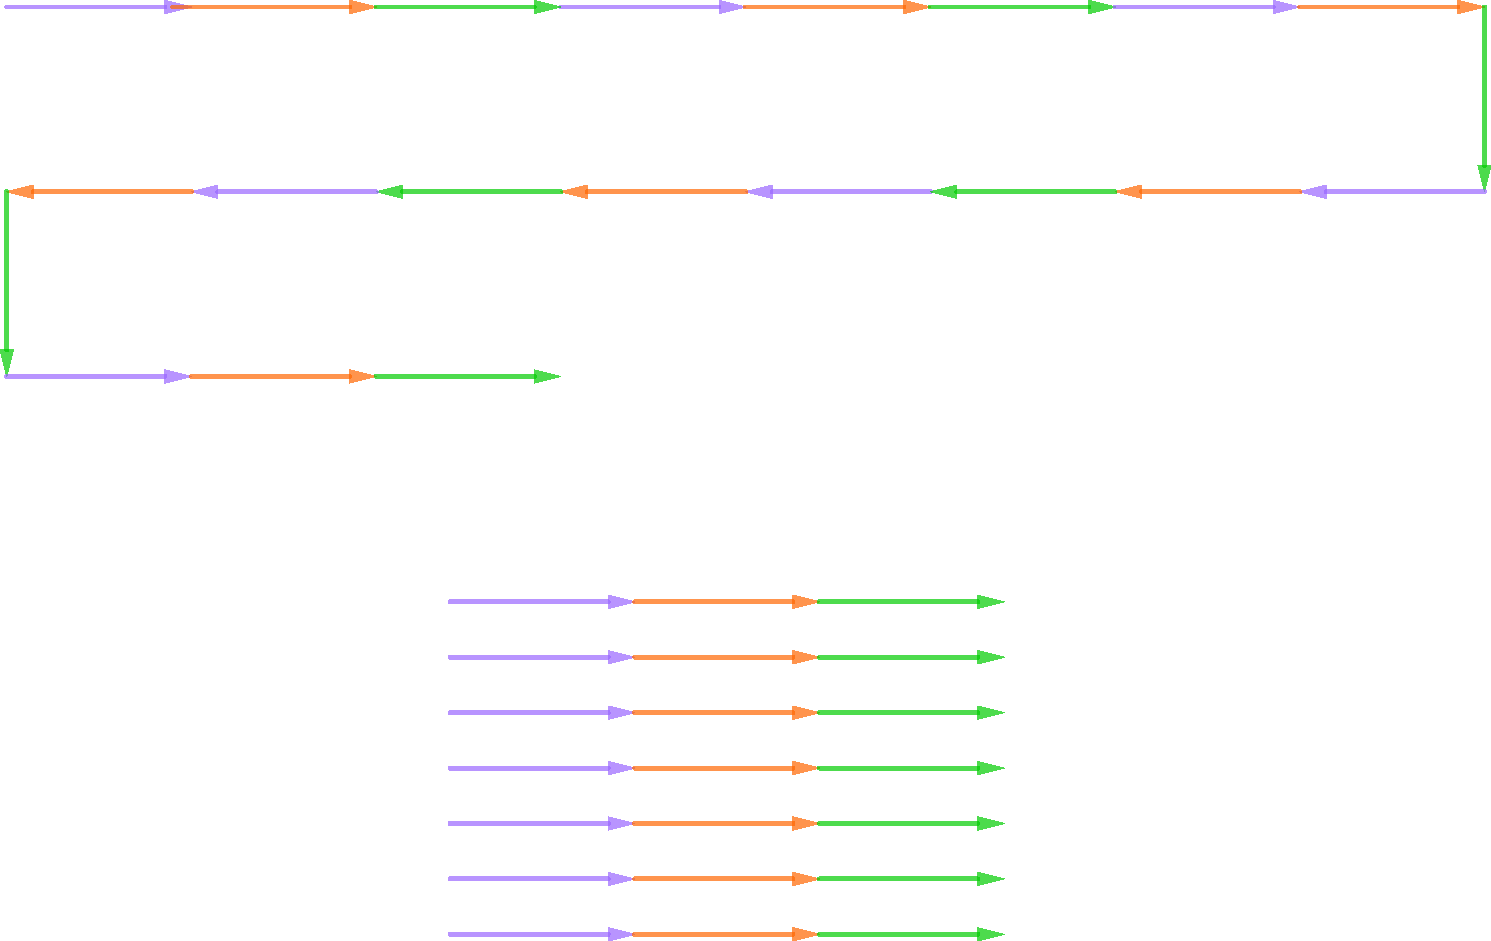
\includegraphics[scale=0.2]{figures/criticalPath.pdf}
	\end{figure}
\end{frame}

\section{Parallel computing}
\begin{frame}{A world of buffers}
	The aim of parallel computing is solving heavy arithmetic computation on buffer. It's independent operations base on a large amount of data. One process is call a kernel for the GPGPU or a shader for the graphic pipeline.
	\begin{figure}
		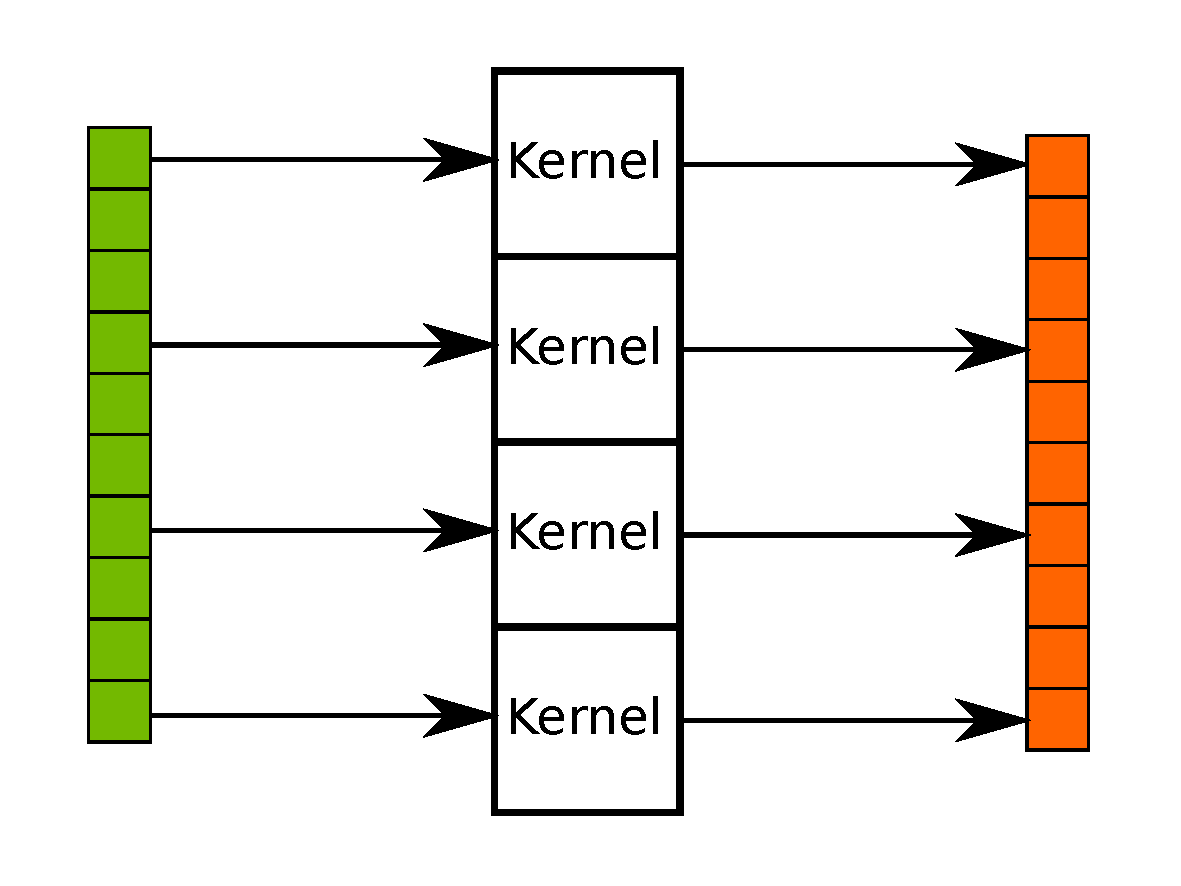
\includegraphics[scale=0.3]{figures/buffer.pdf}
	\end{figure}
\end{frame}

\section{What is a video card?}
\begin{frame}{History}
	At the beginning (1970) a Graphics Processing Unit (GPU) is used for drawing game sprite. It was dedicated device for formatted data. Ten years after we have the ability to draw line, fill area and control the blitter. In 1990, graphical API appear allow us to send assembly code to the device.
\end{frame}

\begin{frame}{Arithmetic Logic Unit}
	The Arithmetic Logic Unit (ALU) is the component for performing arithmetic operations. Because GPU is more focused on floating point operations, multiple ALU are combined to create Floating Point Unit (FPU).
	\begin{figure}
		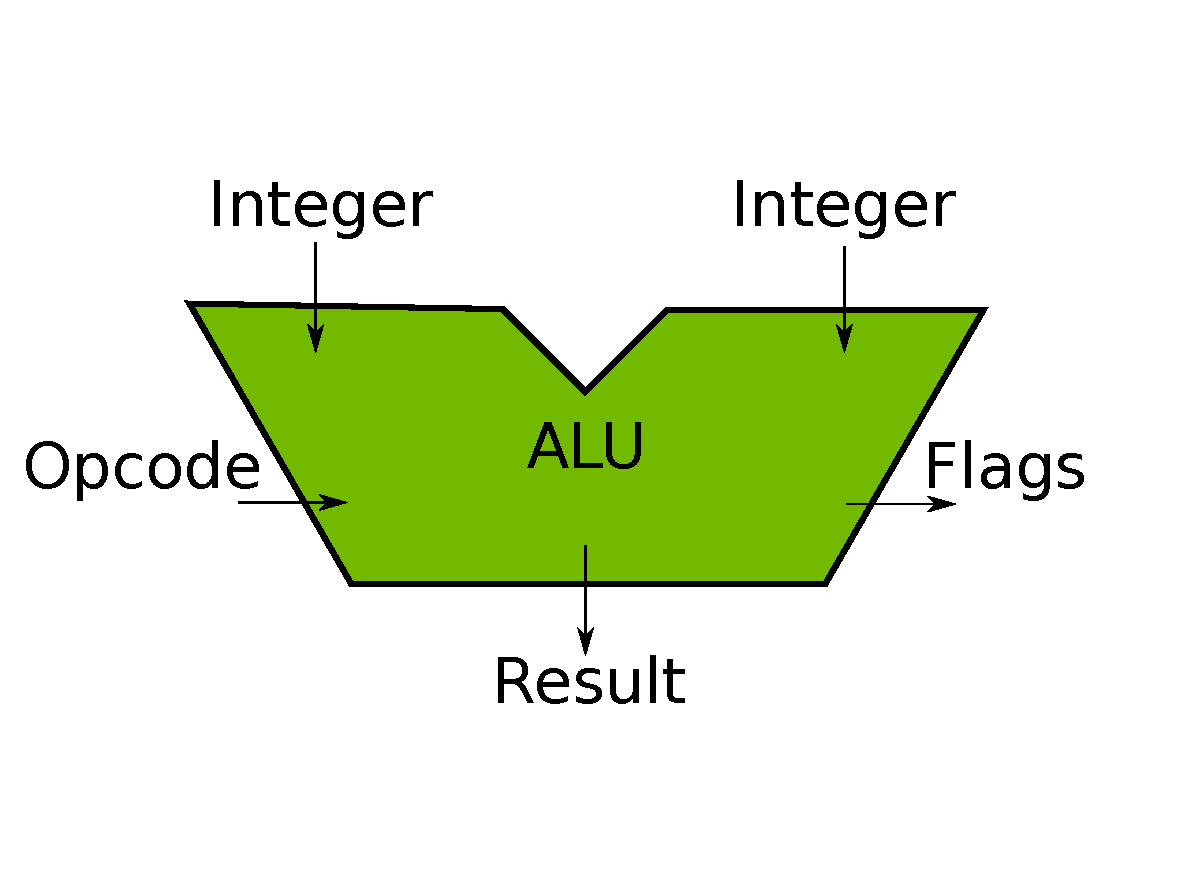
\includegraphics[scale=0.3]{figures/ALU.pdf}
	\end{figure}
\end{frame}

\begin{frame}{CUDA Core}
	CUDA cores are used to execute opcodes from compiled kernels. There are composed of a FPU, a logic unit, branch unit and compare unit.
	\begin{figure}
		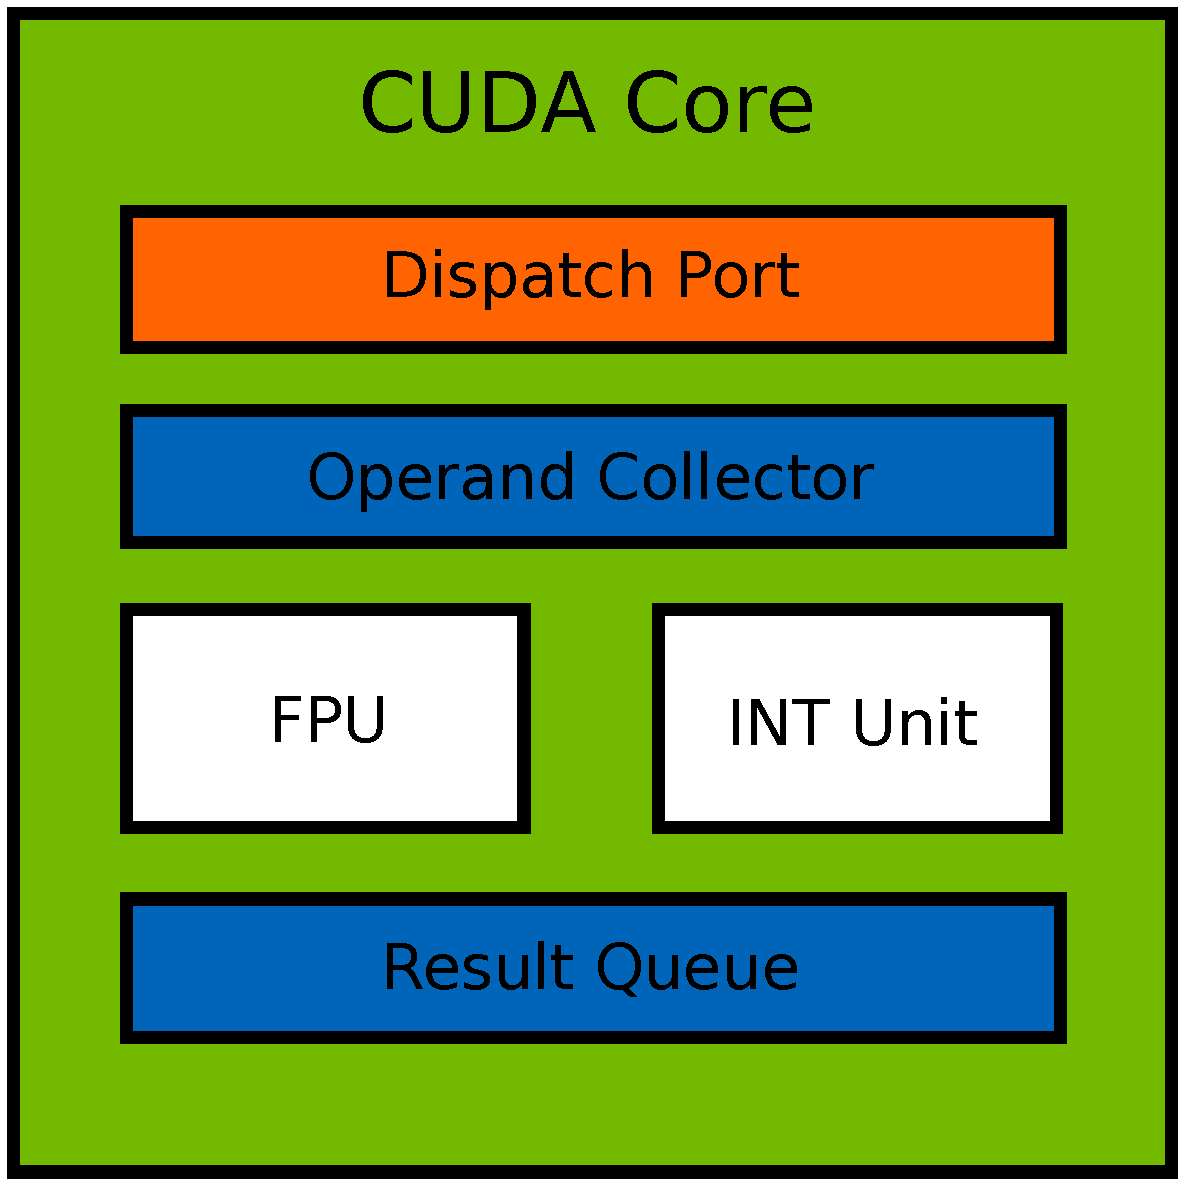
\includegraphics[scale=0.2]{figures/cudacore.pdf}
	\end{figure}
\end{frame}

\begin{frame}{Streaming Multiprocessor}
	Streaming Multiprocessor (SM) organizes threads in groups of 32 called warp. This architecture is called SPMD (Single Program, Multiple Data).
	\begin{figure}
		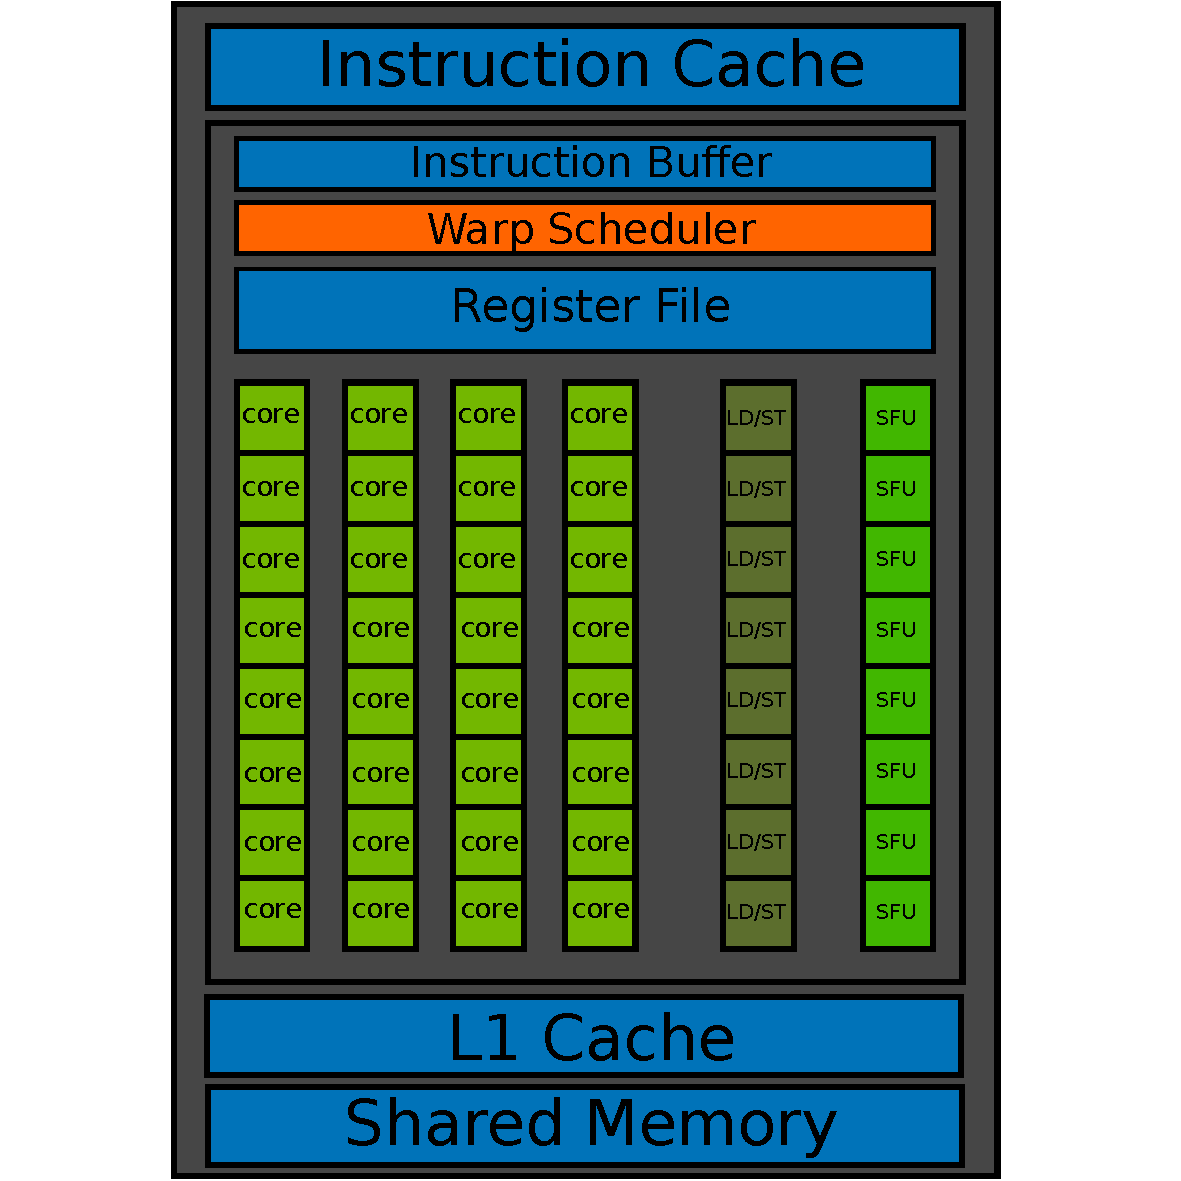
\includegraphics[scale=0.3]{figures/warp.pdf}
	\end{figure}
\end{frame}

\begin{frame}{Streaming Multiprocessor}
	On the GP104 (The GPU of GTX 1080) each SM have 4 warps. 
	\begin{figure}
		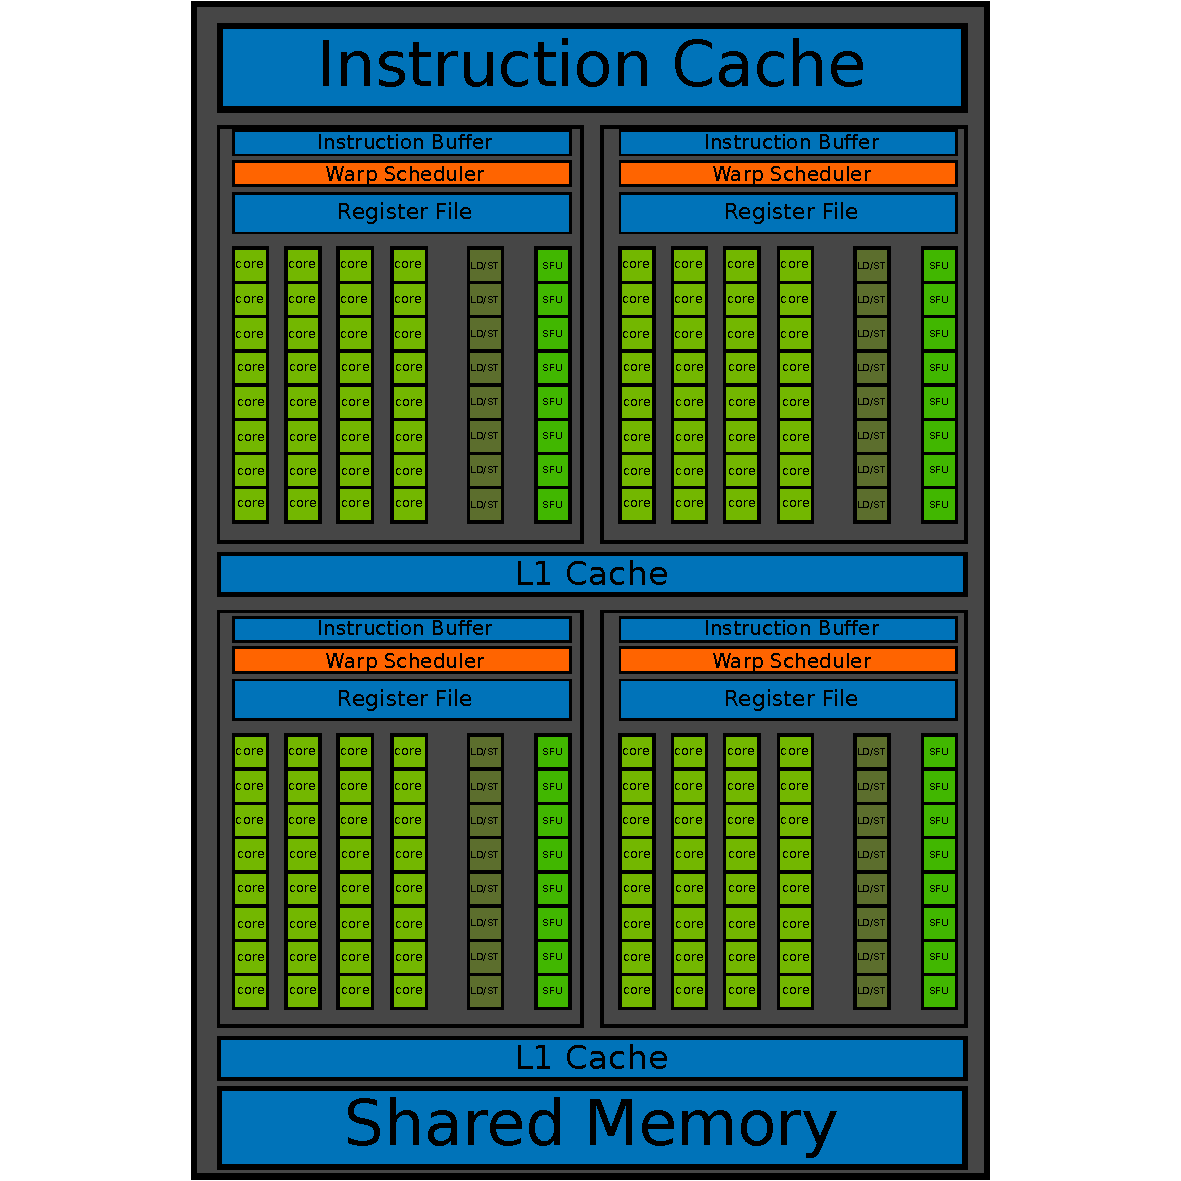
\includegraphics[scale=0.3]{figures/SM.pdf}
	\end{figure}
\end{frame}

\begin{frame}{Graphics Processing Clusters}
	A Graphics Processing Clusters (GPC) is a collection of streaming multiprocessors. In the case of the GP104, there is 4 clusters.
	\begin{figure}
		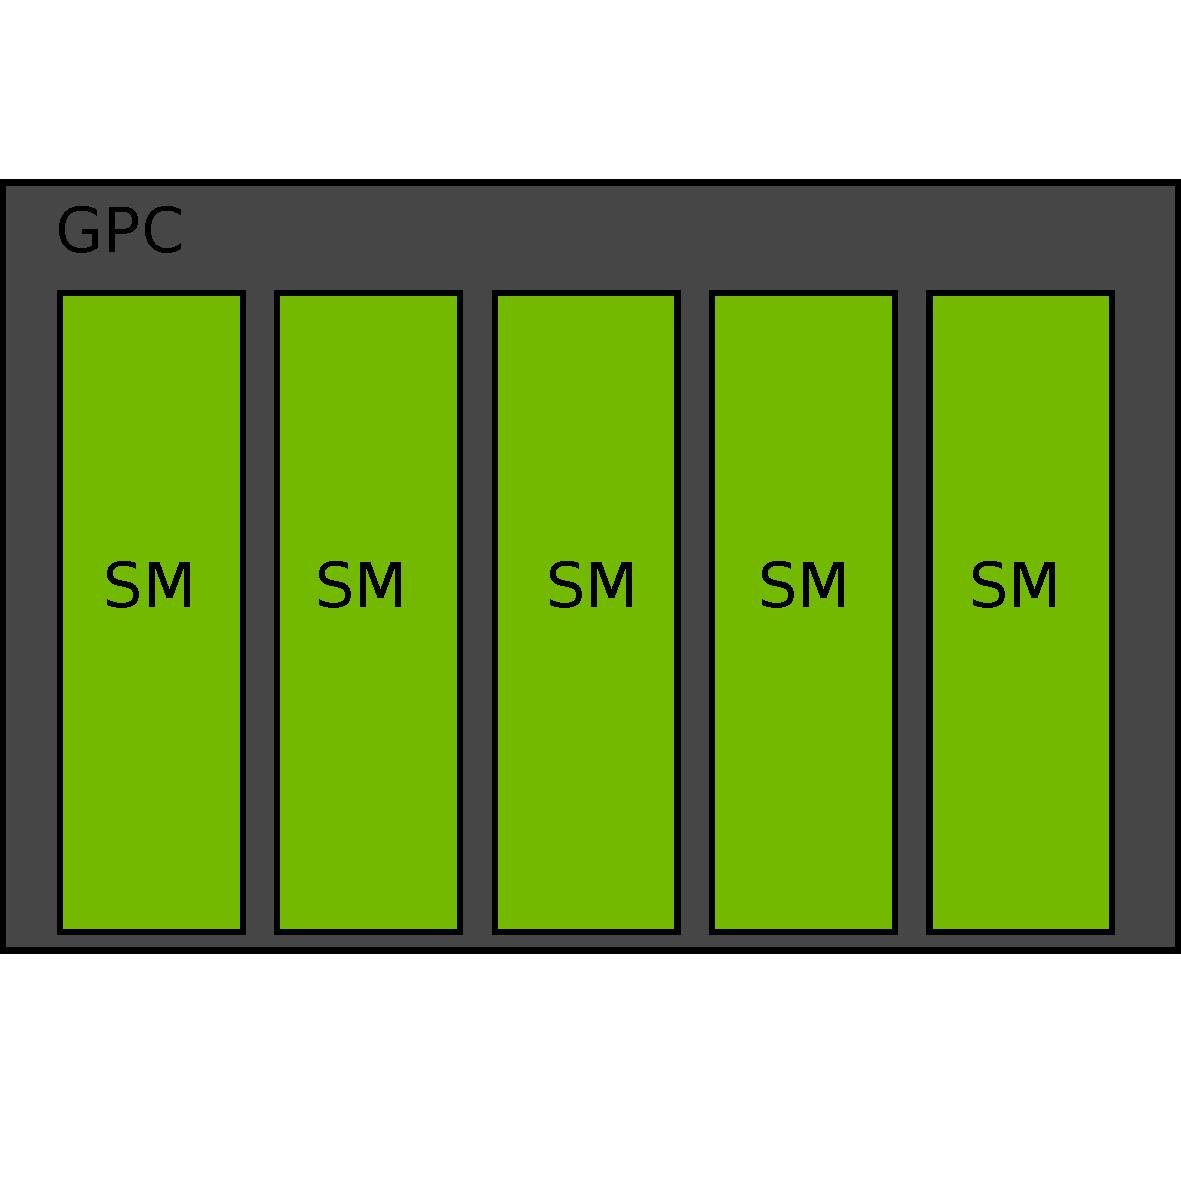
\includegraphics[scale=0.3]{figures/GPC.pdf}
	\end{figure}
\end{frame}

\begin{frame}{GP104}
	All the GPC are connected to the L2 cache memory. The Gigathread engine distribute block threads to Streaming multiprocessor. This device have 32 core * 4 warps * 5 SM * 4 GPC = 2560 CUDA cores
	\begin{figure}
		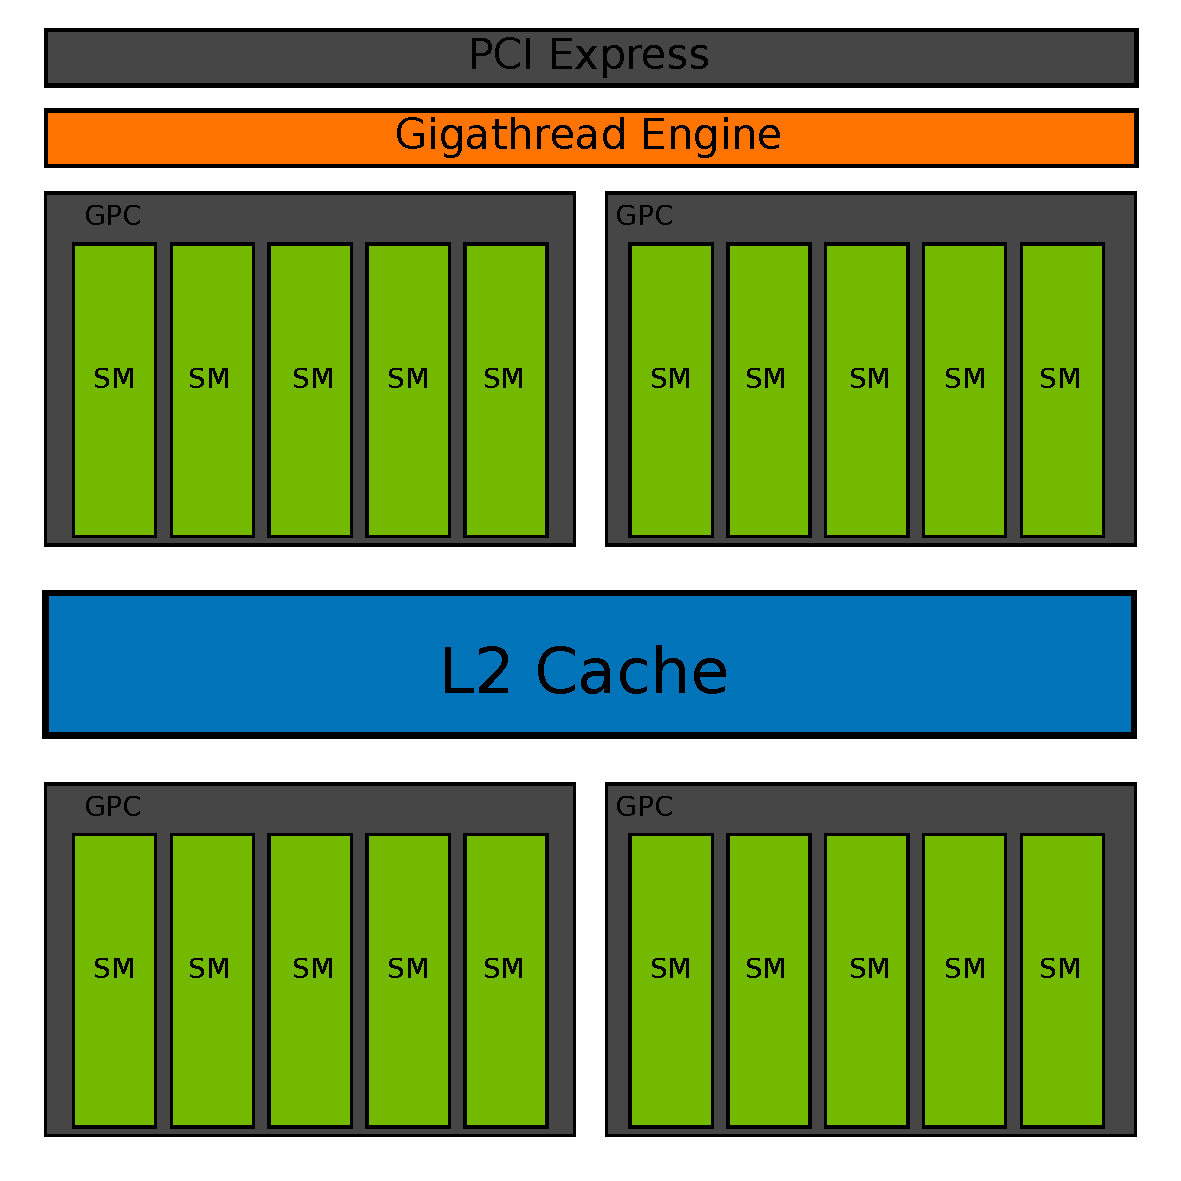
\includegraphics[scale=0.3]{figures/gp104.pdf}
	\end{figure}
\end{frame}

\section{CUDA}
\begin{frame}{Host and Devices}
	\begin{itemize}
		\item Host : The CPU and its memory. The host can manage on both the host and the device. The code executed can launch kernels.
		\item Devices : The GPU and its memory. Kernels are executed on many GPU threads in parallel.
	\end{itemize}
\end{frame}

\begin{frame}{Kernel}
	With CUDA, the kernel declaration is easy. the keyword \_\_global\_\_ have to be added before the kernel function.\\
	The number of thread that execute the kernel is specified by this syntax: \\
	kernelName\textless\textless\textless blocksPerGrid, threadsPerBlock \textgreater\textgreater\textgreater()
\end{frame}

\begin{frame}{Indexing}
	Into the kernel, the threadIdx, the blockIdx and the blockDim allow the user to calculate the index of buffers.\\
	index = blockIdx * blockDim + threadIdx\\
	In the case of data have to be store into 2D or 3D array, it is possible to launch the kernel using a dim3 instead of a int and the index become:\\
	x = blockIdx.x * blockDim.x + threadIdx.x\\
	y = blockIdx.y * blockDim.y + threadIdx.y\\
	z = blockIdx.z * blockDim.z + threadIdx.z\\
\end{frame}

\section{An efficient way to optimize a software}
\begin{frame}{APOD}
	The Assess, Parallelize, Optimize, Deploy(APOD) design cycle goal to identify bottleneck into application. 
\end{frame}

\section{GPGPU usage in the industry}
\begin{frame}{GPGPU usage in the industry}
	
\end{frame}

\end{document}
